\section{Perturbaciones}
\label{sec:perturbaciones}

Las perturbaciones se priorizaron según cuánto afectan a un multirrotor
pequeño en la práctica: viento primero, interferencia electromagnética en el
magnetómetro después y cambios de masa o carga en tercer lugar.
\cod{disturbances.py} las implementa en ese orden,
más una falla parcial de motor. Todas se configuran en
\cod{DisturbanceConfig} y se actualizan una vez por periodo de control.
También pueden agregarse durante la simulación (por ejemplo, desde la GUI):
\cod{DisturbanceManager.add\_payload\_event} y \cod{add\_motor\_fault} agregan
eventos programados, y \cod{Simulation.attach\_payload} aplica una carga de
inmediato.

\subsection{Viento}

La velocidad del viento en $\E$ es la suma de un viento medio, una
turbulencia y una ráfaga discreta:
\begin{equation}
\vect v_w(t)=\underset{\scriptscriptstyle \text{medio}}{-V_m\begin{bmatrix}\cos\chi\\ \sin\chi\\ 0\end{bmatrix}}
+\vect u_{turb}(t)+\vect v_{rafaga}(t),
\label{eq:viento}
\end{equation}
con $\chi$ la dirección \emph{de donde} sopla (un viento ``del norte'',
$\chi=0$, empuja hacia el sur, $-x_E$). Entra a la dinámica solo como
velocidad del aire en \eqref{eq:vrel}.

\paragraph{Turbulencia de Dryden.} El modelo de Dryden (MIL-F-8785C
\cite{mil8785}, MIL-HDBK-1797 \cite{milhdbk1797}) describe la turbulencia
como ruido blanco filtrado con espectros dados. El simulador usa un filtro
formador de \emph{primer orden} por eje (proceso de Gauss--Markov),
\begin{equation}
\dot u=-\frac{V}{L}\,u+\sigma\sqrt{\frac{2V}{L}}\;n(t),
\label{eq:dryden}
\end{equation}
cuya varianza estacionaria es $\sigma^2$ y cuyo tiempo de correlación es
$L/V$. Se integra por Euler--Maruyama con el paso de control. A baja altura
($h<1000$~ft) las escalas de longitud son las de la norma,
\begin{equation}
L_w=h,\qquad L_u=L_v=\frac{h}{(0.177+0.000823\,h)^{1.2}}\quad(h\ \text{en pies}),
\end{equation}
y la intensidad vertical se toma como $\sigma_w=0.5\,\sigma$, que es lo que
da la relación de la norma, $\sigma_w/\sigma_u=(0.177+0.000823h)^{0.4}=\val{dryRatio}$,
a 1.5~m. La velocidad que fija el ancho de banda es
$V=\max(\|\vect v\|,V_m,1~\text{m/s})$.

La verificación (bloque K, 3000~s simulados a 1.5~m con $V_m=3$~m/s y
$\sigma=1$~m/s) da una desviación de \val{drySu}~m/s en $u$ y \val{drySw}~m/s
en $w$, una escala $L_u=\val{dryL}$~m y un tiempo de correlación medido
(caída a $1/e$ de la autocorrelación) de \val{dryTm}~s, frente al teórico
$L/V=\val{dryTc}$~s.

\begin{supuesto}[Simplificaciones de la turbulencia]
La norma especifica para $v$ y $w$ espectros de segundo orden (con un cero),
y define $u$ a lo largo del viento medio; aquí los tres ejes usan el primer
orden y van alineados con NED. Para un multirrotor que vuela a pocos m/s,
con escalas de decenas de metros, la diferencia está en el extremo de alta
frecuencia del espectro, que el arrastre del fuselaje ya filtra. La
intensidad $\sigma$ se da directamente en m/s, sin la tabla de probabilidad
de excedencia de la norma.
\end{supuesto}

\paragraph{Ráfaga discreta $1-\cos$.} Entre $t_0$ y $t_0+d$,
\begin{equation}
v_{rafaga}(t)=\frac{A}{2}\left(1-\cos\frac{2\pi(t-t_0)}{d}\right),
\label{eq:rafaga}
\end{equation}
en la dirección de la que viene la ráfaga: sube a $A$ en $d/2$ y vuelve a
cero, como la ráfaga discreta de la norma militar. La \cref{fig:viento}
muestra una realización.

\begin{figure}[H]
\centering
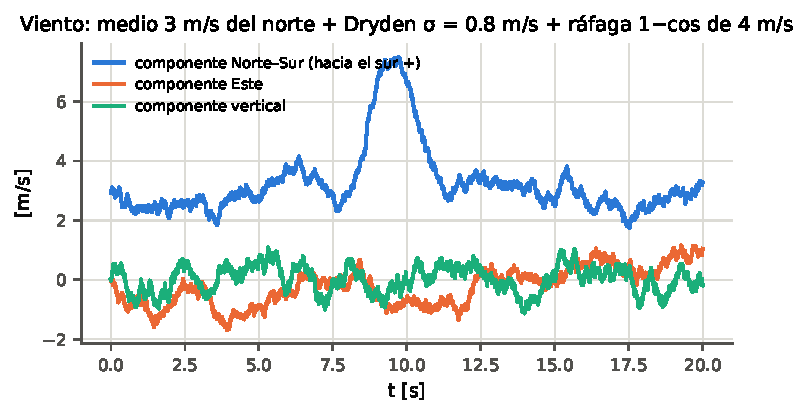
\includegraphics[width=0.85\textwidth]{viento_dryden.pdf}
\caption{Viento medio de 3~m/s del norte, turbulencia de Dryden con
$\sigma=0.8$~m/s y ráfaga $1-\cos$ de 4~m/s entre 8 y 11~s.}
\label{fig:viento}
\end{figure}

\subsection{Interferencia electromagnética en el magnetómetro}

Las corrientes de los ESC y del cableado de potencia generan un campo que
se suma al terrestre en el magnetómetro. El modelo
(\cod{DisturbanceManager.\_emi}) lo hace proporcional a una corriente
equivalente:
\begin{equation}
\vect b_{EMI}=k_I\left(\frac14\sum_i\sigma_i^{1.5}\right)\hat{\vect d}_{EMI}+\text{pulsos},
\label{eq:emi}
\end{equation}
con $k_I=15~\mu$T (campo con los cuatro motores a fondo),
$\hat{\vect d}_{EMI}=(0.6,0.8,0)$ en el cuerpo y pulsos opcionales de
amplitud uniforme en $\pm30~\mu$T a una tasa dada (por ejemplo, un servo).
En hover ($\sigma_h=\val{sigmah}$) el campo parásito es \val{emiH}~$\mu$T, el
\val{emiRel}~\% de la componente horizontal del campo terrestre; si el
estimador confiara solo en el magnetómetro, el rumbo se desviaría
\val{emiPsi}$^\circ$. Es la razón por la que PX4 ofrece compensación del
magnetómetro por corriente (\cod{CAL\_MAG\_COMP}). La perturbación afecta
solo a la medida.

\begin{supuesto}[El exponente 1.5]
El comentario del código justifica $\sigma^{1.5}$ como ``potencia de la
hélice $\propto\Omega^3$''. Esa equivalencia vale si el empuje fuera
proporcional al acelerador ($\Omega\propto\sqrt\sigma$), pero en el modelo de
propulsor de este simulador $\Omega$ es afín en $\sigma$
(\cref{eq:esc}); con él, la corriente de fase sería $\propto\Omega^2$ y la de
batería $\propto\Omega^3$. El exponente es por tanto una forma funcional
supuesta, no derivada; como $k_I$ es un parámetro libre de la
perturbación, la discrepancia solo cambia cómo crece la interferencia con el
acelerador.
\end{supuesto}

\subsection{Cambio de masa y carga útil}

Un evento a un tiempo $t$ engancha (o suelta) una masa puntual $m_p$ en la
posición $\vect r$ del cuerpo (\cod{vehicles.with\_payload}). La carga cambia
tres cosas, y las tres le importan al control:
\begin{gather}
m'=m+m_p,\qquad \vect c'=\frac{m\,\vect c+m_p\,\vect r}{m'},\qquad
\vect d_0=\vect c-\vect c',\qquad \vect d=\vect r-\vect c',\label{eq:carga}\\
J'_{xx}=J_{xx}+m(d_{0,y}^2+d_{0,z}^2)+m_p(d_y^2+d_z^2)\quad\text{(y análogos, teorema de Steiner)},\nonumber
\end{gather}
donde $\vect c$ es el centro de masa actual medido en el marco geométrico del
bastidor (cero en el vehículo nominal, distinto de cero si ya había cargas)
y $\vect r$ la posición de la nueva carga en ese mismo marco. Así varias
cargas sucesivas se componen correctamente: cada una traslada el tensor
acumulado al nuevo centro de masa común. Los brazos de palanca de los rotores pasan a medirse desde el nuevo
centro de masa, $(x_i-c'_x,\ y_i-c'_y)$. Solo se conserva la diagonal del
tensor: los productos de inercia que introduce una carga descentrada se
desprecian. El controlador y el mezclador \emph{no se enteran}: siguen
usando el vehículo nominal, que es lo que pasa en un dron real al que se le
cuelga algo.

\begin{table}[H]
\centering
\small
\caption{Efecto de una carga de 300~g en el PAE-X450 (bloque K).}
\label{tab:carga}
\begin{tabularx}{\textwidth}{lXX}
\toprule
& Carga en $(0,0,5)$~cm (debajo) & Carga en $(5,0,0)$~cm (adelante) \\
\midrule
$J_{xx},J_{yy},J_{zz}$ [kg·m$^2$] & \val{plJz} & \val{plJx} \\
Desplazamiento del centro de masa & \val{plCMz}~mm en $z$ & 8.82~mm en $x$ \\
Momento en hover con aceleradores iguales & 0 & \val{plMy}~N·m (morro abajo) \\
Momento normalizado que debe aportar el integrador & 0 & \val{plU} \\
Acelerador de hover & \val{plSig} & \val{plSig} \\
\bottomrule
\end{tabularx}
\end{table}

La carga descentrada produce un momento constante que solo un término
integral puede compensar; la centrada solo cambia la masa y la inercia,
es decir, la ganancia de la planta. Por eso el escenario de carga de los
bancos de comparación (300~g en $(4,4,5)$~cm, enganchada en $t=8$~s) mide a
la vez robustez a la ganancia y rechazo de perturbación.

\subsection{Pérdida de eficiencia de un motor}

A partir de un instante dado, la velocidad de régimen del motor $i$ se
multiplica por $\eta_i<1$ en \eqref{eq:rotor}. Con $\eta=0.8$ el rotor da el
64~\% del empuje para el mismo acelerador. El controlador lo ve como una
perturbación de momento y de empuje que debe absorber con su integrador.

\subsection{Escenarios estándar}

Para que todos los experimentos sean comparables, \cod{scenarios.py} define
cuatro escenarios con nombre: \emph{nominal}; \emph{viento} (3~m/s del
norte, Dryden $\sigma=1$~m/s, ráfaga de 4~m/s del este en $t=6$~s durante
2~s); \emph{carga} (300~g descentrada en $t=8$~s); y \emph{EMI} (15~$\mu$T a
plena potencia más pulsos de 30~$\mu$T a 0.5~Hz).
